%
%tabbasis, tab1, tab2 -
\subsection{Dampfdruck}
Aus Gleichung (\ref{eqdruck}) und (\ref{eqwstrich}) lässt sich zur jeweiligen Temperatur
der Dampfdruck $p_{\text{sät}}$ und die mittlere freie Weglänge $\overline w$ bestimmen 
(Tab. \ref{tabbasis}). Der Abstand zwischen Kathode und Beschleunigungselektrode beträgt 
bei der Apparatur etwa a=1cm \cite{anleitung}. 

\begin{table}[h]
\begin{center}
\begin{tabular}[c]{cccc} 
a / $\overline w$&$\overline w$ /m & $p_{sät}$ /bar & T /K\\ \hline
2&$ 5,95\cdot 10^{-3}$ &  4,87$\cdot 10^{-6}$& 297,1\\ 
305&$ 3,28\cdot 10^{-5}$ &  8,85$\cdot 10^{-4}$& 383,2\\
1481&$ 6,75\cdot 10^{-6}$ &  4,30$\cdot 10^{-3}$& 420,2\\ 
6060&$ 1,65\cdot 10^{-6}$ &  1,75$\cdot 10^{-2}$& 459,7 
\end{tabular}
\caption{Mittlere Weglänge und Dampfdruck in Abhängigkeit der Temperatur}
\label{tabbasis}
\end{center}
\end{table}

\subsection{Differentielle Energieverteilung der Elektronen} \label{kap1}
\begin{table}[h]
	\begin{center}
		\begin{tabular}{cc}
			$U_A$ / V& $I_A$ / nA\\ \hline
			0,0&	14,50\\
			0,5&	14,35\\
			1,0&	14,30\\
			1,5&	15,30\\
			2,0&	14,25\\
			2,5&	14,20\\
			3,0&	14,16\\
			3,5&	14,12\\
			4,0&	14,01\\
			4,5&	13,92\\
			5,0&	13,82\\
			5,5&	13,73\\
			6,0&	13,59\\
			6,5&	13,35\\
			7,0&	13,06\\
			7,5&	12,78\\
			8,0&	12,35\\
			8,5&	11,64\\
			9,0&	10,59\\
			9,5&	5,32\\
			10,0&	0,14
		\end{tabular}
		\caption{Wertepaare der integralen Energieverteilung($T=23,9^{\circ}$ C)}
		\label{tab1}
	\end{center}
\end{table} \begin{table}[h]
	\begin{center}
		\begin{tabular}{cc}
			$U_A$ / V& $I_A$ / nA\\ \hline
			0,00&	1,15\\
			0,25	&1,05\\
			0,50	&1,00\\
			0,75	&0,96\\
			1,00	&0,89\\
			1,25	&0,84\\
			1,50	&0,78\\
			1,75	&0,71\\
			2,00	&0,65\\
			2,25	&0,59\\
			2,50	&0,57\\
			2,75	&0,46\\
			3,00	&0,39\\
			3,25	&0,33\\
			3,50	&0,26\\
			3,75	&0,21\\
			4,00	&0,15\\
			4,25	&0,10\\
			4,50	&0,07\\
			4,75	&0,04\\
			5,00	&0,02
		\end{tabular}
		\caption{Wertepaare der integralen Energieverteilung($T=147^{\circ}$ C)}
		\label{tab2}
	\end{center}
\end{table}
Mit dem XY-Schreiber wurde der Auffängerstrom $I_A$ in Abhängigkeit von
der Bremsspannung $U_A$ bei zwei verschiedenen Temperaturen ($T_1$ = 23,9 $^{\circ}$ C, 
$T_2$ = 147 $^{\circ}$ C) aufgenommen. Die Beschleunigerspannung $ U_B $ wurde auf 10 V eingestellt. 
Der maximal erreichte Auffängerstrom betrug $I_1=14,5$ nA und $I_2=1,15$ nA.
Aus den aufgezeichneten Messkurven lassen sich die Werte in Tabelle \ref{tab1} und Tabelle \ref{tab2}) 
ablesen. Dabei wurde $\Delta U_{A,1}=0,5$ V und $\Delta U_{A,2}=0,25$ V gewählt. Da $U_A$ nicht
linear anwächst, wird jeweils für die Bereiche, welche von Spannungsmesswerten begrenzt sind,
eine eigene lineare Normierung der Größe der 1 cm-Quadratkästchen des Millimeterpapiers bestimmt (Tab. \ref{tabnorm}).
Dabei wird mit $U_{A,\text{links}}$, $U_{A,\text{rechts}}$ der linke, beziehungsweise rechte Rand 
des Abstandes a zwischen den Spannungsmesswerten bezeichnet, woraus sich dann das Verhältnis von
Kästchengröße zu Spannungsdifferenz, $b=\Delta U_A / 1$ cm, ergibt. Für die Stromstärke sind nur 
zwei Werte aufgezeichnet worden, weshalb eine hier eine lineare Normierung angenommen wird. Für 
$T_2$ ist der Graph um 1 mm nach oben verschoben, erkennbar an der Asymptotik für große $U_A$, was
ebenfalls in die Normierung mit einfließt.
\begin{align}
\text{Abstand von }I_0 \text{ bis }I_1: a_{I,1}&=15,2\text{ cm} \\
\Rightarrow b_{I,1}&=\Delta I_ {A,1}/a_{I,1}=0,95\frac{nA}{ cm} \\
\text{Abstand von }I_0 \text{ bis }I_2: a_{I,2}&=13,9\text{ cm} \\
\Rightarrow b_{I,2}&=\Delta I_ {A,2}/a_{I,2}=0,083\frac{nA}{ cm}
\end{align}

\begin{table}[h]
\begin{center}
\begin{tabular}[c]{cc|cc|cc} 
$U_{A,\text{links}}$ /V & $U_{A,\text{rechts}}$ /V &$a_1$/ cm&$a_2$/ cm& $b_1$ /(V/ cm)& $b_2$ /(V/cm)\\ \hline
0&2&4,25&5,70&0,471&0,351\\
2&4&4,15&5,90&0,482&0,339\\
4&6&4,45&5,90&0,449&0,339\\
6&8&4,50&6,05&0,444&0,331\\
8&10&4,7& - &0,426& - 
\end{tabular}
\caption{Normierung der Messwertaufzeichnung}
\label{tabnorm}
\end{center}
\end{table}

Wird nun $I_A(U_A) - I_A(U_A+\Delta U_A)$ gegen $U_A$ aus Tabelle \ref{tab1}, beziehungsweise 
Tabbelle \ref{tab2}, aufgetragen (Abb. \ref{fig1}, \ref{fig2}),
so entspricht dies, basierend auf Gleichung (\ref{eqbla}), der differentiellen Energieverteilung der
Elektronen bei der jeweiligen Temperatur und es lässt sich für $T_1$ ein Maximum bei $U_{eff}=9$ V ablesen.
Daraus lässt sich das Kontaktpotential bestimmen, $K=U_B-U_{eff}=10\text{ V }-9\text{ V }=1$ V.\\

Abbildung \ref{fig1} und Abbildung \ref{fig2} sind mit PyLab basierend auf Python mit Hilfe der 
Matplotlib erstellt worden.

\begin{figure}[h]
	\centering
		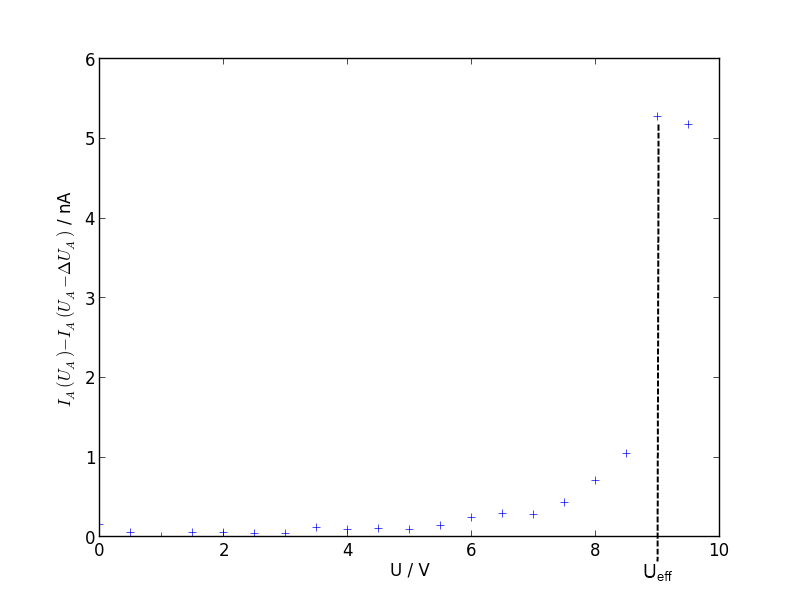
\includegraphics[width=1.00\textwidth]{fig1.png}
		\caption{Energieverteilung der Elektronen bei $T_1$}
	\label{fig1}
\end{figure}

\begin{figure}[h]
	\centering
		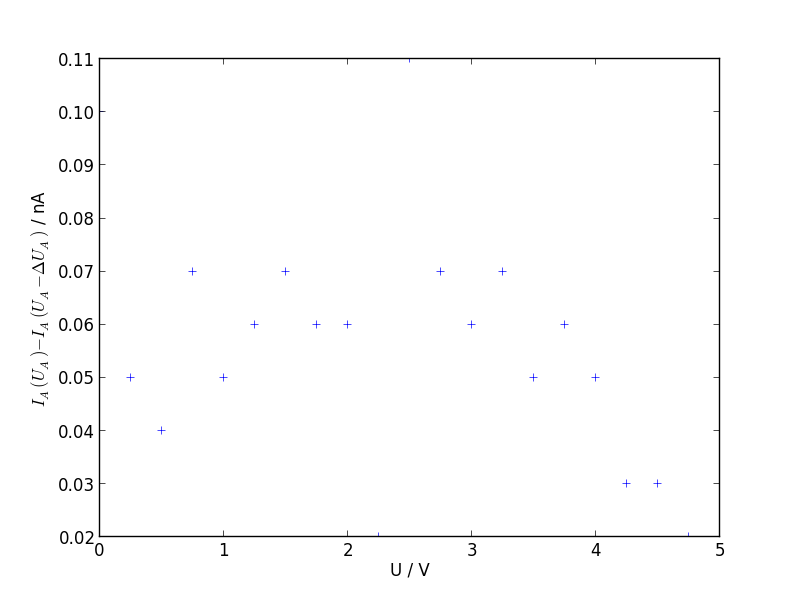
\includegraphics[width=1.00\textwidth]{fig2.png}
		\caption{Energieverteilung der Elektronen bei $T_2$}
	\label{fig2}
\end{figure}

\FloatBarrier

\subsection{Franck-Hertz-Kurve}

Aus der aufgezeichneten Franck-Hertz-Kurve mit $U_A=1$ V bei $T=186,5^{\circ}$ C (Anhang) lässt sich die Lage der $n$ Auffängerstrommaxima
ablesen (Tabelle \ref{tabmax}). Dabei verhält sich die Skalierung der Spannungsachse bis 40 linear, so dass das Verhältnis
von Millimeterpapierskalierung $s$ zur Spannung $U_B$ wie folgt normiert werden kann: 
\begin{align}
c&=\frac{\Delta U_B}{\Delta s}=\frac{40\text{ V}}{16,7\text{ cm}}=2,40\frac{V}{cm}.
\Delta U_B&=U_{B,n}-U_{B,n-1}
\end{align}
Aus Gleichung (\ref{equ1}) kann dann die erste Anregungsenergie des Hg-Atoms berechnet werden (Tab. \ref{tabmax}).

\begin{table}[h]
\begin{center}
\begin{tabular}[c]{ccc} 
n&$U_{B,I max}$ / V&$E_1-E_0$ / eV\\ \hline
1&6,3& - \\
2&11,1&4,8	\\
3&15,7&4,6	\\
4&20,4&4,7	\\
5&25,3&4,9	\\
6&30,1&4,7	\\
7&35,2&5,1	\\
8&40,2&5,0	\\
9&45,5&5,3\\ \hline
&Mittelwert&4,89$\pm$0,08
\end{tabular}
\caption{Maxima der Franck-Hertz-Kurve}
\label{tabmax}
\end{center}
\end{table}

Aus dem errechneten Mittelwert der ersten Anregungsenergie wird die beim Übergang in den Grundzustand
emittierte Wellenlänge $\lambda$ berechnet (Gl. (\ref{eqlambda}) bzw. Gl. (\ref{eqlicht})).
\begin{align}
\lambda&=c\frac{h}{E_1-E_0}= (254\pm4)\text{nm , $c$: Lichtgeschwindigkeit}\label{eqlambda}
\end{align}


\subsection{Ionisation}
Zum Ermitteln der Ionisationsspannung $U_i$ wird aus der Kurve mit konstanter Abbremsspannung von 
$U_A=-30$ V bei einer Temperatur von $T=110^{\circ}$ C (Anhang) der Wert $U_i+K=12$ V extrapoliert.
Mit dem in \ref{kap1} bestimmten Wert für $K$ lässt sich $U_i=11$ V bestimmen.
